\section{Theorie}
\label{sec:Theorie}

\subsection{Brechung und Dispersion}
Durchdringt ein Lichtstrahl eine Grenzfläche in ein Medium mit anderer Dichte, so wird die Richtung des Lichtstrahls geändert. In Abbildung 1
ist dieser Effekt zu sehen.

\begin{figure}[H]
  \centering
  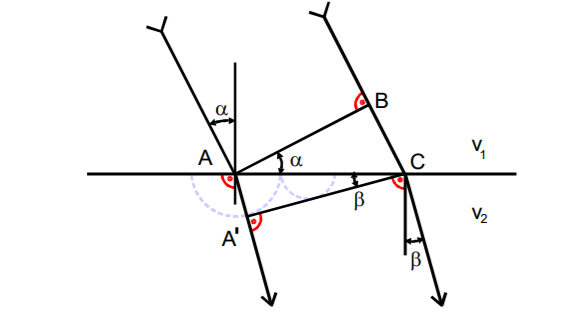
\includegraphics[height=5cm]{wellenfront.PNG}
  \caption{Brechung von Lichtstrahlen an einer Wellenfront \cite{sample}}
  \label{fig:biegungbild1}
\end{figure}

Für die Brechungswinkel $\alpha$ und $\beta$ und den Brechungsindex $n = \frac{v_1}{v_2}$ gilt:
\begin{align}
  n = \frac{\sin{\alpha}}{\sin{\beta}}
\end{align}
 Dabei sind $v_1$ und $v_2$ die Geschwindigkeiten von Licht in den jeweiligen Medien.

Lichtgeschwindigkeit in Medien ist eine frequenzabhängige Größe. Dieses Phänomen wird Dispersion genannt.

Werden Elektronen und Ionenrümpfe in der Materie berücksichtigt, kann eine Dispersiongleichung abgeleitet werden. Die
eltektrischen Ladungen und Ionenrümpfe, befinden sich in einer Gleichgewichtslage. Das E-Feld der Lichgwellen regt diese
zu Schwingungen an, wodurch auch Resonanzerscheinungen auftreten. Durch die verschobenen Ladungsträger, wegen der Lichtwellen, wird
eine rücktreibende Kraft, sowie eine dämpfnede Reibung, induziert. Für die bewegung der Ladungsträger kann eine Differentialgleichung
formuliert werden.
\begin{align}
  m_h \frac{\symup{d}^2 \vec{x}_h}{\symup{d}t^2} + f_h \frac{\symup{d} \vec{x}_h}{\symup{d}t} + a_h \vec{x}_h = q_h \vec{E}_0 e^{i\omega t}
\end{align}

Hierbei ist $m_h$ die Teilchenmasse,  $q_h$ die Ladung, $\vec{E}_0$ das E-Feld,  $a_h$ die Beschleunigung,  $\omega$ die Kreisfrequenz.
Für $f_h$ gilt die Beziehung $\vec{F}_{D,h} = f_h \frac{\symup{d} \vec{x}_h}{\symup{d}t}$ mit der Reibung $\vec{F}_{D,h}$.

Mit dieser Differentialgleichung lässt sich eine Beziehung für den komplexen Brechungsindex $\tilde{n}$ und der Lichtfrequenz herleiten.
\begin{align}
  \tilde{n}^2 = 1+ \sum_{h} \frac{1}{\omega_h^2 - \omega^2 + i \frac{f_h}{m_h}\omega} \frac{N_q q_h^2}{m_h \epsilon_0}
\end{align}

Zwischen $\tilde{n}$ und $n$ gilt dann die Beziehung:
\begin{align}
\tilde{n} = n(1-ik)
\end{align}

Mit der Absorptionskonstante $k$ des Lichtes in Materie. Das Modell der erzwungenen Schwingung kann nur ausreichend beschrieben werden, wenn die
Dispersionskurve weit außerhalb der der Resonanzstellen betrachtet wird. Es soll gelten $n^2 k \approx 0$. Aus Gleichung (3) folgt dann eine
Beziehung zwischen Brechungsindex und Wellenlänge:
\begin{align}
  {n}^2 (\lambda) = 1+ \sum_{h} \frac{1}{4 \pi c^2 \epsilon_0 m_h} \frac{\lambda^2 \lambda_h^2}{\lambda^2-\lambda_h^2}
\end{align}


\subsection{Fallunterscheidungen für die Resonanzstelle}
Besitzt die betrachtete Materie nur eine Absorptionstelle $\lambda_1$ so kann eine Fallunterscheidung gemacht werden.
Fall a:Für $\lambda \gg \lambda_1$ kann Gleichung (5) entwickelt werden.
\begin{align}
  {n}^2 (\lambda) = 1 + \frac{N_1 q_1^2 \lambda_1^2}{4 \pi c^2 \epsilon_0 m_1} \left(1+ \left(\frac{\lambda_1}{\lambda}\right)^2
  + \left(\frac{\lambda_1}{\lambda}\right)^4 + ... \right)
\end{align}

Mit Koeffizienten $A_i > 0$ kann die Gleichung auch wie folgt ausgedrückt werden:
\begin{align}
  {n}^2 (\lambda) = A_0 + \frac{A_2}{\lambda^2} + \frac{A_4}{\lambda4} + ...
\end{align}


Fall b: Für  $\lambda \ll \lambda_1$ gilt:
\begin{align}
  {n}^2 (\lambda) = 1 + \frac{N_1 q_1^2}{4 \pi c^2 \epsilon_0 m_1} \left(\lambda^2+ \frac{\lambda^4}{\lambda_1^2}
  + \frac{\lambda^6}{\lambda_1^4} + ... \right)
\end{align}

Oder mit Koeffizienten $A_i' > 0$ , $i \geq 2$
\begin{align}
  {n}^2 (\lambda) = 1 - A_2' \lambda^2 - A_4' \lambda^4 - ...
\end{align}

\begin{figure}[H]
  \centering
  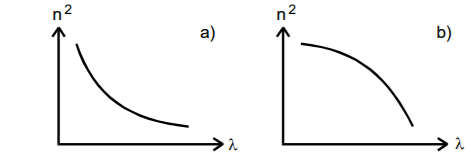
\includegraphics[height=4cm]{dispersion.PNG}
  \caption{Dispersionskurve der beiden Fälle \cite{sample}}
  \label{fig:biegungbild1}
\end{figure}

In beiden Fällen sinkt der Brechungsindex mit steigender Wellenlänge. Dieses Verhalten wird als Normale Dispersion bezeichnet.
